%\documentclass[handout,xetex,notheorems,hyperref={pdfpagelabels=true},xcolor={table}]{beamer}
\documentclass[xetex,notheorems,hyperref={pdfpagelabels=true},xcolor=table]{beamer}
\usetheme{minflat}
\usepackage{booktabs}
\usepackage[scale=2]{ccicons}
\usepackage{hyperref}
\usepackage[style=american]{csquotes}
\usepackage{soul}
\usepackage{xcolor}
\usepackage{listings}
\usepackage{xskak,chessboard}
\usepackage{pgfpages}
\setbeamertemplate{caption}[numbered]
\usetikzlibrary{decorations.pathreplacing, decorations.pathmorphing,calc,arrows,positioning}

%%% enable notes on second screen
%\usepackage{pgfpages}
%\setbeameroption{show notes on second screen=right}
%\setbeamertemplate{note page}[compress]
\usepackage{tikz,tikzpeople,forest}
%%%%%%%%%%%%%%%%%%%%%%%%%%%%%%%%%%%%%%%%%%%%%%%%%%%
%%%%	define content of title page
%%%%%%%%%%%%%%%%%%%%%%%%%%%%%%%%%%%%%%%%%%%%%%%%%%%
\def\talkTitle{Cybernetics}
%\def\talkShortTitle{}
%\def\talkSubtitle{}
\def\talkKeywords{Sonos, Ugur Turhal, University of Basel}
\newcommand{\eg}[1]{\textit{e.}\textit{g. }}
%% Define meta data of pdf
\hypersetup{
    pdftitle={Slides to talk - \talkTitle},
	pdfsubject={\talkTitle},
	pdfauthor={Ugur Turhal},
	pdfkeywords={\talkKeywords},
	colorlinks=false
}

\makeatletter
\let\HL\hl
\renewcommand\hl{%
  \let\set@color\beamerorig@set@color
  \let\reset@color\beamerorig@reset@color
  \HL}
\makeatother
%%%%%%%%%%%%%%%%%%%%%%%%%%%%%%%%%%%%%%%%%%%%%%%%%%%
%%%%	set content of title page
%%%%%%%%%%%%%%%%%%%%%%%%%%%%%%%%%%%%%%%%%%%%%%%%%%%
\title[\talkShortTitle]{\talkTitle}  
%\subtitle{\talkSubtitle} 
\author{Ugur Turhal -- \href{mailto:ugur.turhal@unibas.ch}{ugur.turhal@unibas.ch} \\ Mario Tachikawa -- \href{mailto:mario.tachikawa@unibas.ch}{mario.tachikawa@unibas.ch}}
\DTMlangsetup[en-GB]{ord=raise,monthyearsep={,\space}}
\vspace*{0.25cm}
\date{\DTMtoday}
\institute{%
	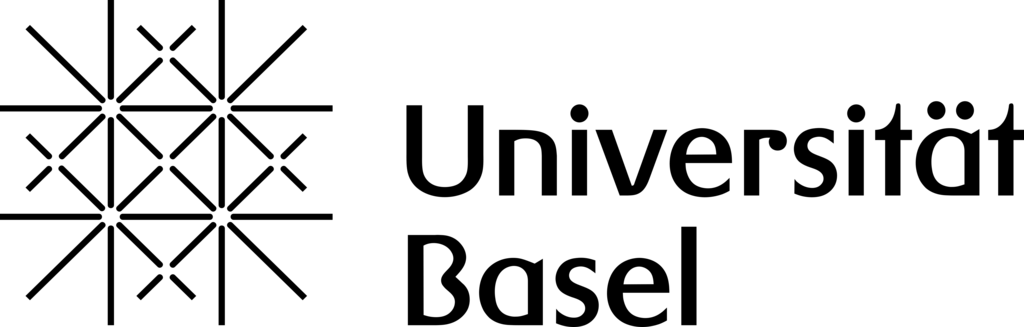
\includegraphics[width=.3\textwidth]{./gfx/logo.png}%
}
\usetikzlibrary{shapes,arrows,fit,calc,positioning}
  \tikzset{box/.style={draw, diamond, thick, text centered, minimum height=0.5cm, minimum width=1cm}}
  \tikzset{line/.style={draw, thick, -latex'}}
%%%%%%%%%%%%%%%%%%%%%%%%%%%%%%%%%%%%%%%%%%%%%%%%%%%
%%%%	theorem tools, theorem and proof styles
%%%%%%%%%%%%%%%%%%%%%%%%%%%%%%%%%%%%%%%%%%%%%%%%%%%
\setbeamertemplate{theorem}[ams style]
%\setbeamertemplate{theorems}[numbered]

\newcounter{chapter}
\setcounter{chapter}{1}
\theoremstyle{plain}
\newtheorem{theorem}{Theorem}[section]
\newtheorem{lemma}[theorem]{Lemma}
\newtheorem{proposition}[theorem]{Proposition}
\newtheorem{corollary}[theorem]{Corollary}

\theoremstyle{definition}
\newtheorem{conclusion}[theorem]{Conclusion}
\newtheorem*{definition}{Definition}
\newtheorem*{remark}{Remark}
\newtheorem*{dummyblock}{dummyblock}

\theoremstyle{example}
\newtheorem*{example}{Conclusion}

\theoremstyle{example}
\newtheorem*{example2}{SOAP - Structure}

%\newenvironment<>{dummyblock}[1]{%
%	\setbeamercolor{block title}{fg=white,bg=white}%
%	\setbeamercolor{block body}{fg=normal text.fg,bg=yellow}%
%	\begin{block}#2{#1}}{\end{block}}

\mode<handout>{
\usepackage{pgfpages}
\usepackage{tikz,tikzpeople}
  \pgfpagesuselayout{4 on 1}[a4paper,landscape,border shrink=5mm]
  \setbeamertemplate{background canvas}{
    \begin{tikzpicture}[remember picture]
      \draw[darkpurple] (current page.south west) rectangle (current page.north east);
    \end{tikzpicture}
    }
}
\begin{document}

\definecolor{olive}{rgb}{1.0, 0.88, 0.21}

\renewcommand{\leq}{\leqslant}
\renewcommand{\geq}{\geqslant}
\renewcommand<>\cellcolor[1]{\only#2{\beameroriginal\cellcolor{#1}}}
\renewcommand\theta\vartheta
\DeclareRobustCommand{\hlcyan}[1]{{\sethlcolor{cyan}\hl{#1}}}
\DeclareRobustCommand{\hlolive}[1]{{\sethlcolor{olive}\hl{#1}}}
%%%%%%%%%%%%%%%%%%%%%%%%%%%%%%%%%%%%%%%%%%%%%%%%%%%
%%%%	title page
%%%%%%%%%%%%%%%%%%%%%%%%%%%%%%%%%%%%%%%%%%%%%%%%%%%
%{\usebackgroundtemplate{%
  %\includegraphics[width=0.49\textwidth]{gfx/wordcloud.png}}}
\begin{frame}[plain]
	\titlepage
\end{frame}

%%%%%%%%%%%%%%%%%%%%%%%%%%%%%%%%%%%%%%%%%%%%%%%%%%%
%%%%	toc
%%%%%%%%%%%%%%%%%%%%%%%%%%%%%%%%%%%%%%%%%%%%%%%%%%%
%\begin{frame}
%	\tableofcontents
%\end{frame}

%\imageFrameOverlayLeft{%
%./gfx/wordcloud.png}{%
%Sonos advertises}{with}
%%%%%%%%%%%%%%%%%%%%%%%%%%%%%%%%%%%%%%%%%%%%%%%%%%%
%%%%	introduction
%%%%%%%%%%%%%%%%%%%%%%%%%%%%%%%%%%%%%%%%%%%%%%%%%%%
\section{Introduction}
\begin{frame}{Characteristics}
Characteristics of living systems: Power to learn, power to reproduce themselves.
\begin{figure}
    \centering
    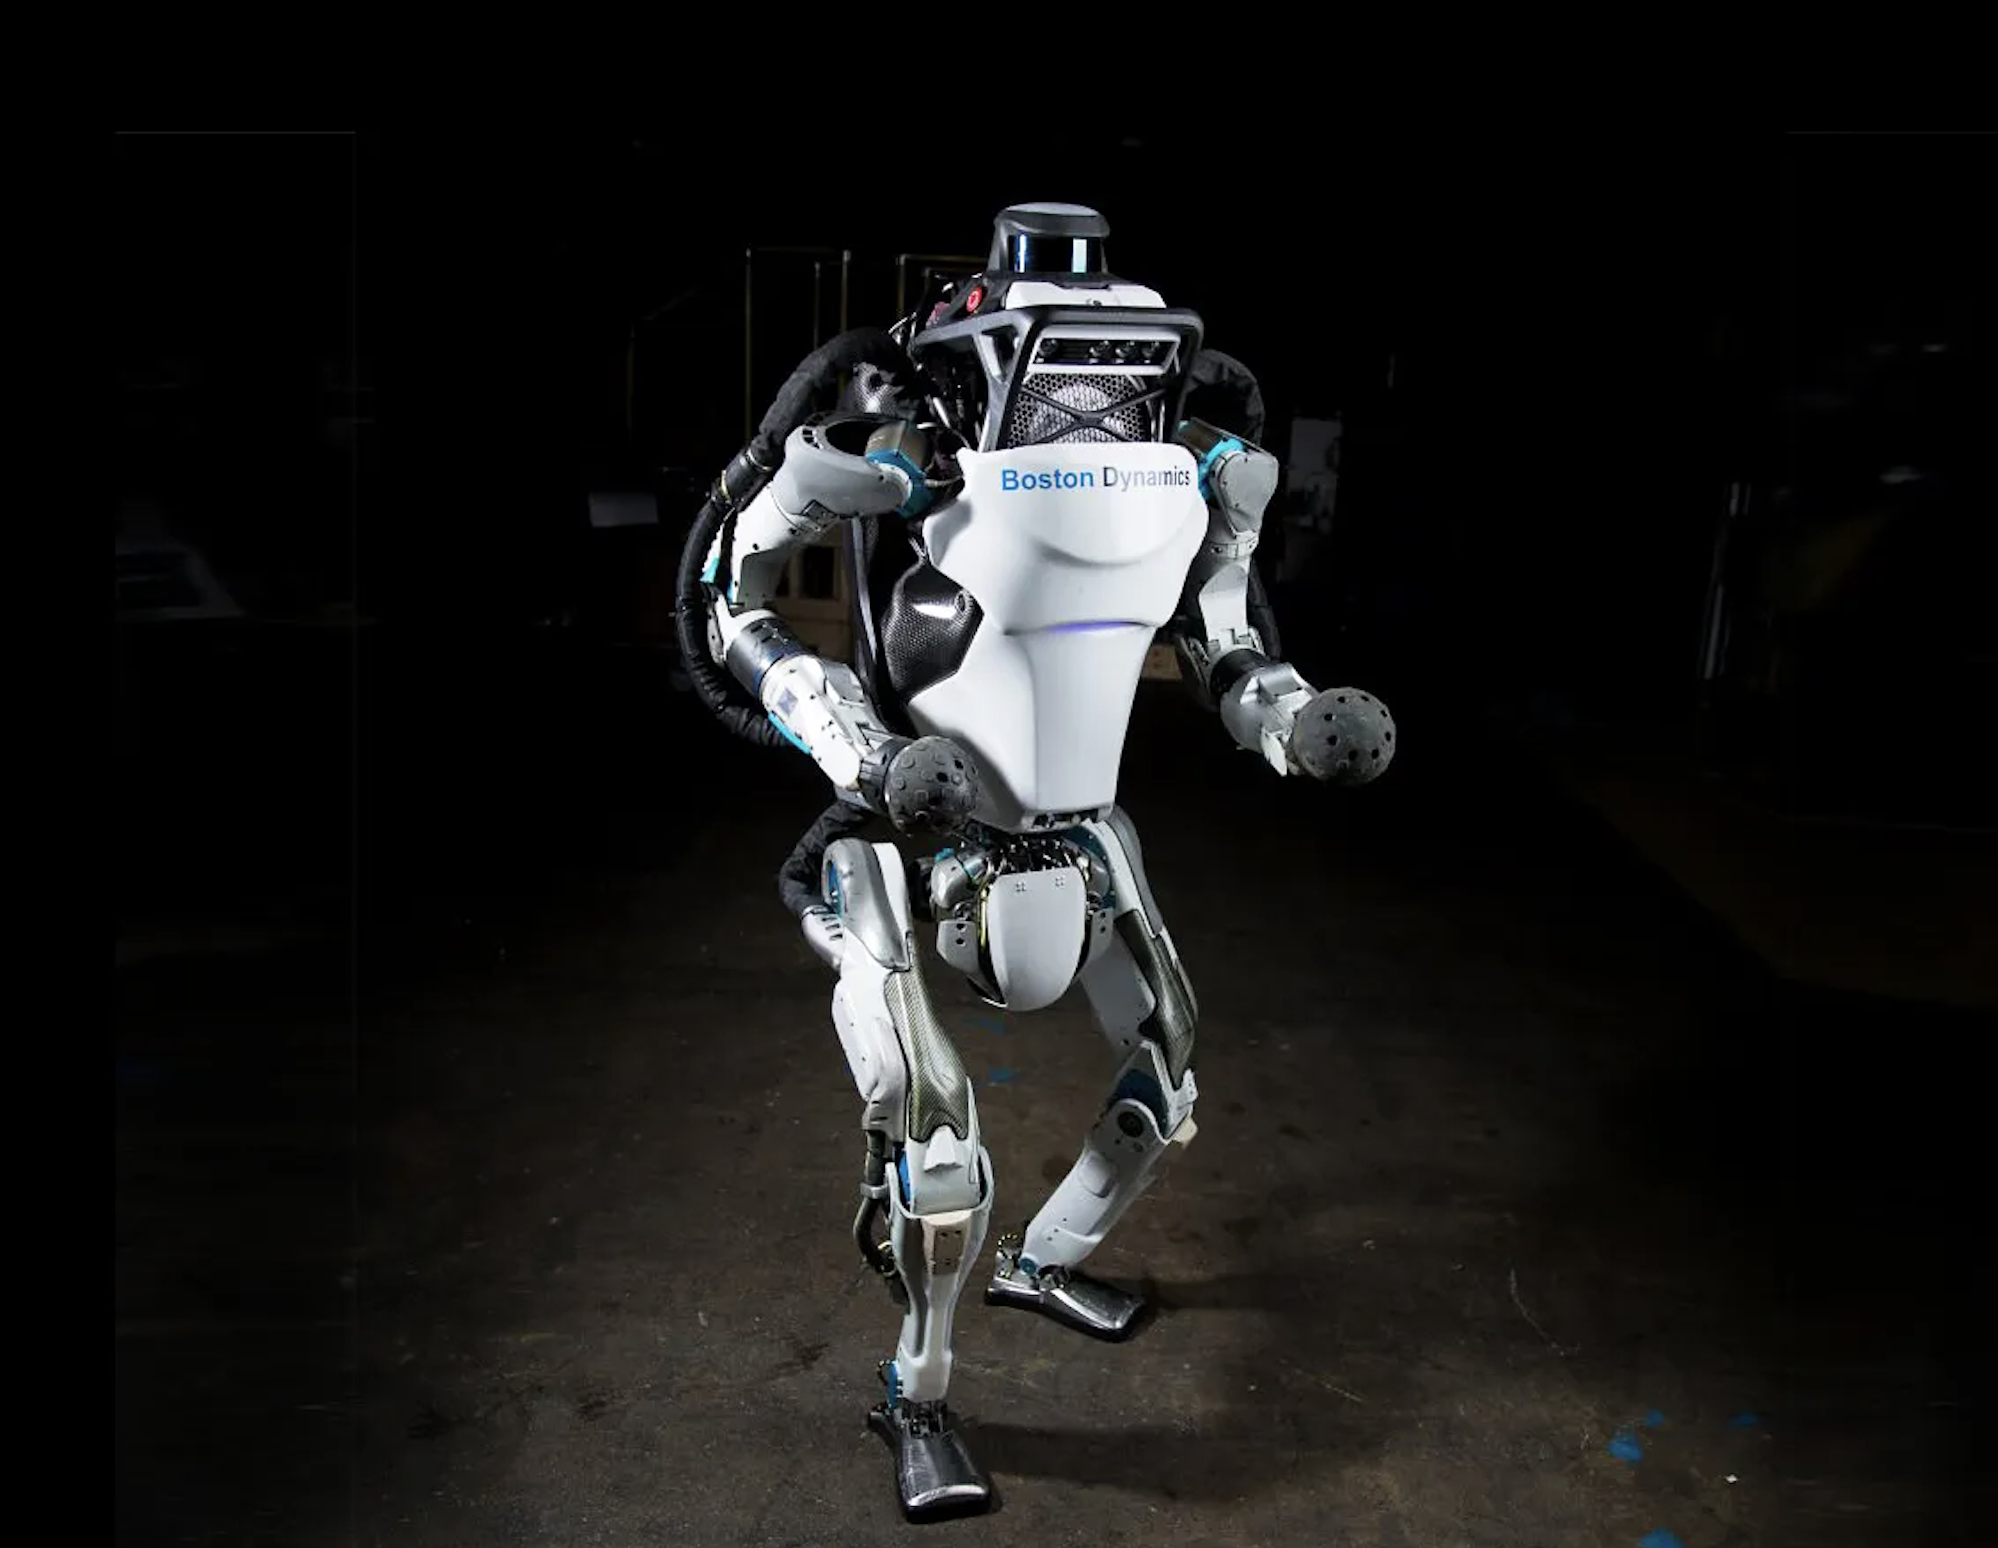
\includegraphics[width=0.49\textwidth]{png/atlas.png}
    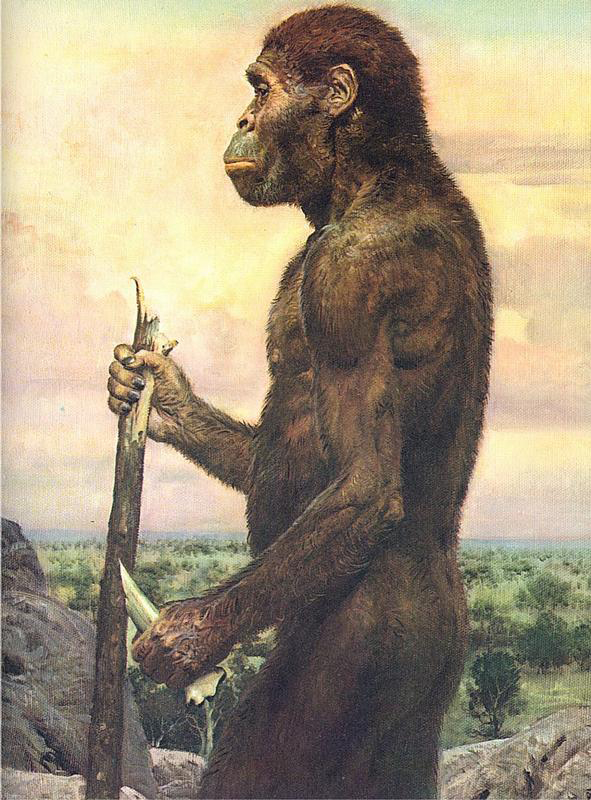
\includegraphics[width=0.49\textwidth, height=4.1cm]{png/urmensch.jpg}
    \caption{Atlas versus Living System}
    \label{fig:enter-label}
\end{figure}
\textit{Question:} Can man-made machines learn and reproduce themselves?
\end{frame}

%%%	image frame with overlay left

\begin{frame}{Learning}
\begin{block}{Forms of learning}
\begin{enumerate}[\indent $\blacksquare$]
    \item Ontogenetic Learning: individual adaptability within a lifetime 
    \item phylogenetic Learning: evolutionary changes over generations. 
\end{enumerate}
\end{block}
$\Rightarrow$ Both forms are crucial for organisms to adjust to their environments
\begin{figure}[h]
  \centering
  \begin{tikzpicture}[font=\small,scale=0.9, transform shape]
      %\node[criminal,minimum size=1cm,monitor] (A) at (-5,0){};
      \path (-4,0) node(A) {
\includegraphics[width=1.5cm]{gfx/ancestors.png}};
      \path (-2,0) node(B) {
\includegraphics[width=1.5cm]{gfx/giraffe.png}};
      \path (2,0) node(C) {
\includegraphics[width=1.5cm]{gfx/cricket.png}};
      \path (4,0) node(D) {
\includegraphics[width=1.5cm]{gfx/humming-bird.png}};
    \node[below] at (A.south) (a) {\textbf{Humans}};
    \node[below] at (B.south) (b) {\textbf{Other mammals}};
    \node[below] at (C.south) (c) {\textbf{Insects}};
    \node[below] at (D.south) (d) {\textbf{Birds}};
 \end{tikzpicture}
\end{figure}
\begin{itemize}
    \item[-] Humans \& other mammals, highest point of "learning". 
    \item[-] Insects \& Birds, not good ontogenetic learners $\rightarrow$ Due to demands of flight
\end{itemize}
\end{frame}
\begin{frame}{Von Neumann Theory - 1}
    \begin{enumerate}
        \item Rational Decision making
        \begin{enumerate}
            \item Game players are rational and aim to maximize their benefits.
        \end{enumerate}
        \item Minimax Theorem
        \begin{enumerate}
            \item In games where one player's gain is another's loss, each player tries to minimize the worst possible outcome.
        \end{enumerate}
        \item Strategy and Equilibrium
        \begin{enumerate}
            \item There is a point in some games where players have no reason to change their strategy, considering the strategies of others.
        \end{enumerate}
    \end{enumerate}
    \begin{figure}[h]
  \centering
  \begin{tikzpicture}[font=\small,scale=0.9, transform shape]
      %\node[criminal,minimum size=1cm,monitor] (A) at (-5,0){};
      \path (-4,0) node(A) {
\includegraphics[width=1.5cm]{gfx/mind.png}};
      \path (0,0) node(B) {
\includegraphics[width=1.5cm]{gfx/sinusoid.png}};
      \path (4,0) node(C) {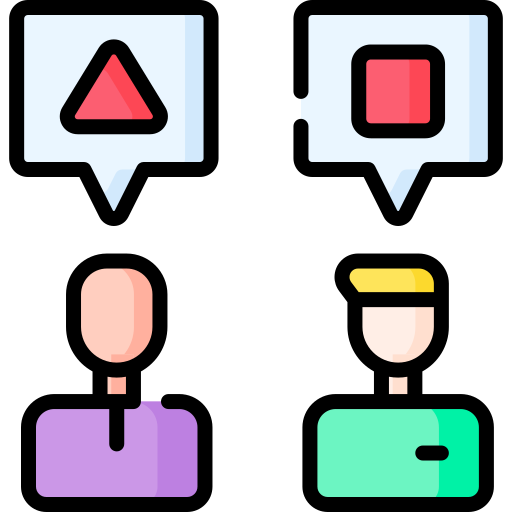
\includegraphics[width=1.5cm]{gfx/point-of-view.png}};
    \node[below] at (A.south) (a) {\textbf{Rational}};
    \node[below] at (B.south) (b) {\textbf{Minmum Maximum}};
    \node[below] at (C.south) (c) {\textbf{Point of view}};
 \end{tikzpicture}
\end{figure}
\end{frame}

\begin{frame}{Von Neumann Theory - 2}
    \begin{enumerate}\addtocounter{enumi}{3}
        \item Game Classification and Solution Concepts
        \begin{enumerate}
            \item Games are categorized by types and rules, which help understand the strategies and outcomes of players' interactions.
        \end{enumerate}
        \item Extensive Form Games and Backward Induction
        \begin{enumerate}
            \item In step-by-step games, players think backward from the end to decide their best moves.
        \end{enumerate}
        \item Applications Beyond Games
        \begin{enumerate}
            \item Von Neumann's game theory is used in various areas, like politics and biology, not just traditional games.
        \end{enumerate}
    \end{enumerate}
    \begin{figure}[h]
  \centering
  \begin{tikzpicture}[font=\small,scale=0.9, transform shape]
      %\node[criminal,minimum size=1cm,monitor] (A) at (-5,0){};
      \path (-4,0) node(A) {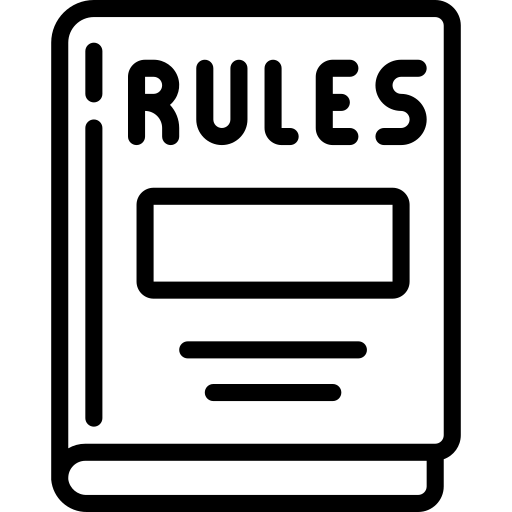
\includegraphics[width=1.5cm]{gfx/book.png}};
      \path (0,0) node(B) {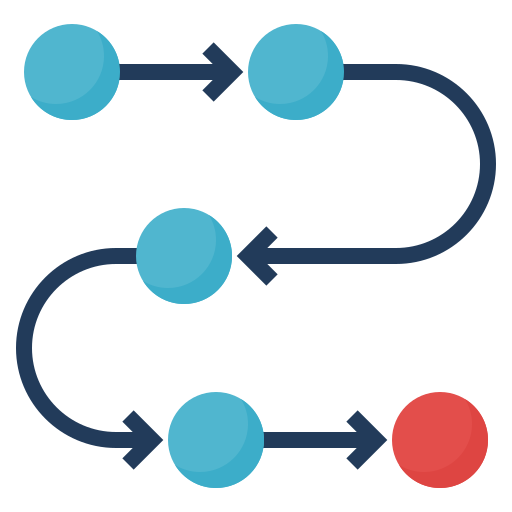
\includegraphics[width=1.5cm]{gfx/process.png}};
      \path (4,0) node(C) {
\includegraphics[width=1.5cm]{gfx/speech.png}};
    \node[below] at (A.south) (a) {\textbf{Rational}};
    \node[below] at (B.south) (b) {\textbf{Minmum Maximum}};
    \node[below] at (C.south) (c) {\textbf{Point of view}};
 \end{tikzpicture}
\end{figure}
\end{frame}

\begin{frame}{Von Neumann always applicable? - NO}
Von Neumann's Theory applies to Tick-Tac-Toe (The entire strategy is known).
    \begin{figure}[h]
  \centering
  \begin{tikzpicture}[font=\small,scale=0.9, transform shape]
      %\node[criminal,minimum size=1cm,monitor] (A) at (-5,0){};
      \path (-4,0) node(A) {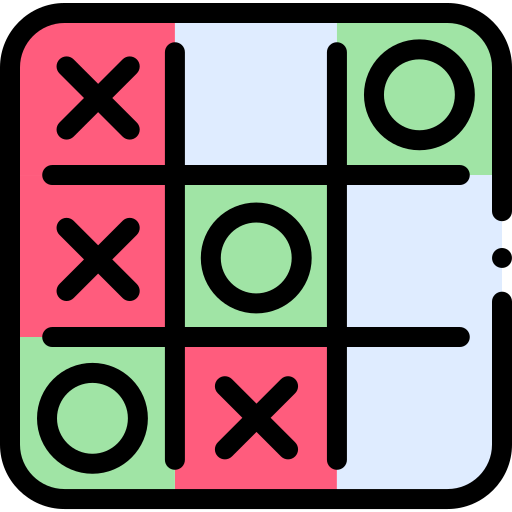
\includegraphics[width=1.5cm]{gfx/tic-tac-toe.png}};
    \node[below] at (A.south) (a) {\textbf{Tic-Tac-Toe}};
 \end{tikzpicture}
\end{figure}
In games like chess, von Neumann's theory can be approximated but not fully applied. (Due to the immense complexity and the vast number of possible positions 
\begin{figure}[h]
\resizebox{.78\totalheight}{!}{
\centering
{\normallineskip=0pt
\setchessboard{smallboard,showmover=false}
\newchessgame
\chessboard}}
\end{figure}
\end{frame}

\begin{frame}{Acting Rational}
Approximating von Neumann's act with the utmost caution and assumption that the opponent is perfectly wise can result in a loss; a loss can also be dangerous and, in war, could be lethal.
\newline \newline Example: Everyday Situation job interview. 
    \begin{figure}[h]
  \centering
  \begin{tikzpicture}[font=\small,scale=0.9, transform shape]
      %\node[criminal,minimum size=1cm,monitor] (A) at (-5,0){};
      \path (-4,0) node(A) {
\includegraphics[width=1.5cm]{gfx/interview.png}};
    \node[below] at (A.south) (a) {\textbf{Job Interview}};
 \end{tikzpicture}
\end{figure}
\begin{enumerate}
    \item Interviewer asks a question.
    \item The person gives a cautious and wise answer. 
    \item Interview Ends
\end{enumerate}
\end{frame}
\section{Game Playing Machines}
\begin{frame}{Game Playing Machines - 1}
\begin{enumerate}[\indent $\square$]
    \item Chess books are not written from a von Neumann point of view.
    \item Making machines that will play chess is not difficult. Ensuring only legal moves are made is well within the capabilities of basic computing machines.
    \item Mobility, pieces, and commands are reduced to numerical terms.
    \item A chess grandmaster, even a "normal" skilled person, can beat such a chess machine. 
    \item But not every chess machine is easy to beat. 
\end{enumerate} 
\end{frame}

\begin{frame}{Game Playing Machines - 2}
\begin{block}{Question}
Can a chess machine learn? Yes, it can.
\end{block}
Taking break $\rightarrow$ Examining previous games (memory), and learning from its "knowledge".\vspace*{0.15cm}\newline
This behavior would also get rid of the rigid personality of the machine.\vspace*{0.15cm}\newline

In chess, each stage of the game (opening, middle, and endgame) requires distinct strategies and move evaluations; thus, a learning machine must adapt its approach to each stage individually to play at a master level.
\vspace*{0.25cm}\newline
In December 2023, the most robust CPU chess engine in the world with an estimated Elo rating of 3546\vspace*{0.25cm}\newline
The best human: 2819 Elo Rating.
\end{frame}

\section{History and Learning}
\begin{frame}{History \& Learning}
\begin{block}{History \& Learning}
Humans learn from history and data (hopefully). Machines also need history and data to forecast/predict the future.
\end{block}
We have two options: First-Order Programming \& Second-Order Programming
    \begin{figure}[h]
  \centering
  \begin{tikzpicture}[font=\small,scale=0.9, transform shape]
      %\node[criminal,minimum size=1cm,monitor] (A) at (-5,0){};
      \path (-3,0) node(A) {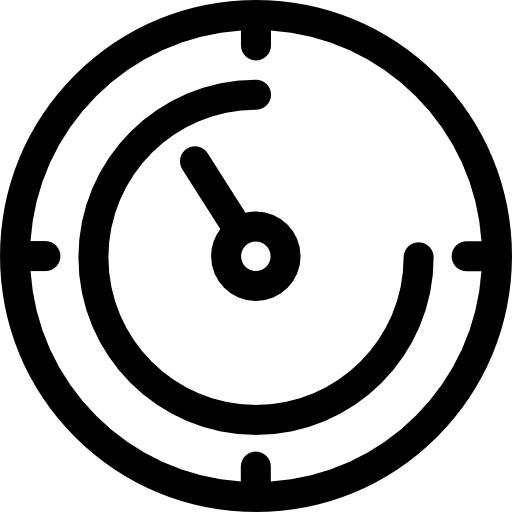
\includegraphics[width=1.5cm]{gfx/thermostat.png}};
      \path (-0,0) node(B) {
\includegraphics[width=1.5cm]{gfx/temperature.png}};
      
    \node[below] at (A.south) (a) {\textbf{Thermostat}};
    \node[below] at (B.south) (b) {\textbf{Smart Thermostat}};
 \end{tikzpicture}
\end{figure}
\begin{enumerate}
    \item A thermostat is an example of linear programming. (Turn on when $\leq$ threshold) Turn off when it is $>$ threshold)
    \item A smart thermostat is an example of nonlinear programming (learns the daily schedule and habits to adjust heating based on current temperature and using historical data for optimal comfort and energy efficiency.)
\end{enumerate}
\end{frame}

\begin{frame}{Curse \& blessing}
    Norbert Wiener: Learning machines are dangerous.
    We must know whether the danger point has come to turn a machine off effectively. Just building does not allow us to judge about the danger point.
    \begin{enumerate}
        \item TODAY: openAI
    \end{enumerate}
    \begin{block}{Quote}
        "A learning machine must be programmed by experience." \\ - Norbert Wiener Page: 244
    \end{block}
    Using learning machines in wars: The values of winning that are employed in the programming games must be the same ones we hold at heart in the actual outcome of a war.
    \vspace*{0.25cm}\newline
    \begin{center}
        $\Rightarrow$ \hl{What we believe to want and what we want differs.}  
    \end{center}
\end{frame}
\section{Reproduction}
\begin{frame}{Reproduction}
Two different perspectives:
\begin{enumerate}
    \item Does a machine have enough parts and a sufficiently complicated structure to enable self-reproduction to be among its functions? $\Rightarrow$ YES.
    \item How to develop a practical method for machines that can replicate themselves?
\end{enumerate}
Second Question use: \textbf{Transducer}. Why transducer? 
\begin{enumerate}
    \item Input - Output %Relationship Crucial for self reproduction. self-reproducing produce a functional response
    \item Good models Complex Systems % models the complex processes involved in self-reproduction
    \item Time Invariance
    \item Simplifying Complex Concepts
    \item Input - (Processing data through a complex, non-linear system) - Output.
\end{enumerate}
\begin{center}
If a machine performs a specific function, then if the input is shifted back in time, the output is shifted back by the same amount.
\end{center}
Crucial for linear aparatus impedance \& admittance, but not suitable for non-linear transducer.
\end{frame}

\begin{frame}{Reproduction 2}
    \begin{block}{Linear versus Non Linear}
        \begin{enumerate}[\indent $\square$]
            \item Linear: Output is direct proportional to input.
            \item Non Linear: Output is not directly proportional to the input example: Microphone. 
        \end{enumerate}
    \end{block}
\begin{enumerate}
    \item Divide Transducers into Smaller Units, Simplify
    \item Same Input to Each Unit, Every smaller unit gets the same input
    \item Sum Outputs for Overall Response Sum the smaller units together for output
    \item Adjust how much each unit contributes to the total output using linear coefficients. 
    \item Linear coefficients are calculated using a method called least-squares, which helps find the best fit, and by averaging the data collected.
\end{enumerate}
$\Rightarrow$ Emulate any non-linear transducer and automatically fine-tune its response. Paralleling biological mechanisms such as gene replication or virus formation, although with distinct technical specifics.
\end{frame}
\section{chapter2}
\begin{frame}{Brain Waves}
% Maybe also say humans are ontogentic, birds are phylgoenetic learners.
    \begin{block}{What are brain waves?}
        \begin{enumerate}[\indent $\blacksquare$]
        \item Electrical patterns in the brain
        \item Generated by activity of neurons
        \item Different brain wave frequencies (\href{https://www.ncbi.nlm.nih.gov/pmc/articles/PMC7176745/#:~:text=These\%20changes\%20can\%20be\%20deduced,(13\%E2\%80\%9020\%20Hz).&text=Delta\%20waves\%20are\%20more\%20frequent\%20during\%20sleep.}{Link})
        \begin{itemize}
            \item $\delta$ = (0-4 Hz), 
            \item $\theta$ = (4-8 Hz), 
            \item $\alpha$ = (8-13 Hz), 
            \item $\beta$ = (13-20 Hz) 
        \end{itemize}
    \end{enumerate}
    \end{block}
\begin{center}
    \begin{tikzpicture}[font=\small,scale=0.9, transform shape]
      %\node[criminal,minimum size=1cm,monitor] (A) at (-5,0){};
      \path (-4,0) node(A) {
\includegraphics[width=1.5cm]{gfx/brain.png}};
      \path (4,0) node(B) {
\includegraphics[width=1.5cm]{gfx/lightning.png}};
      \path (0,0) node(C) {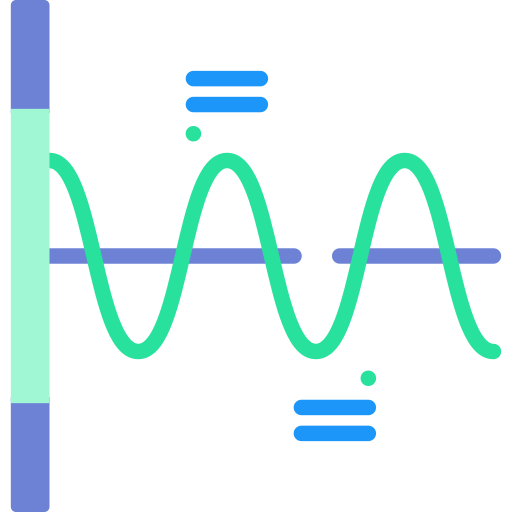
\includegraphics[width=1.5cm]{gfx/waves.png}};
    \node[below] at (A.south) (a) {\textbf{Brain}};
    \node[below] at (B.south) (b) {\textbf{electrical potential}};
    \node[below] at (C.south) (c) {\textbf{Waves}};
 \end{tikzpicture}
\end{center}
 \begin{itemize}
     \item[1.] Brain waves as self-organizing systems 
     \item[2.] Non-linear phenomena
 \end{itemize}

\end{frame}

\begin{frame}{Historical Context and Development of Electrophysiology}
\begin{itemize}
    \item[-] Birth of Electrophysiology: Galvanometers
    \begin{center}
        \begin{tikzpicture}[font=\small,scale=1, transform shape]
             %\node[criminal,minimum size=1cm,monitor] (A) at (-5,0){};
             \path (0,0) node(0);
             \path (7,0) node(A) {
\includegraphics[width=1.5cm]{gfx/galvanometer.png}};
      
            \node[below] at (A.south) (a) {\textbf{Galvanometer}};
    
        \end{tikzpicture}
    \end{center}
    \item[-] Edison's discovery \& cathode-ray oscillograph
    \begin{center}
        \begin{tikzpicture}[font=\small,scale=0.9, transform shape]
             %\node[criminal,minimum size=1cm,monitor] (A) at (-5,0){};
             \path (0,0) node(0);
             \path (7,0) node(A) {
\includegraphics[width=1.5cm]{gfx/oscilloscope.png}};
      
            \node[below] at (A.south) (a) {\textbf{Oscillograph}};
    
        \end{tikzpicture}
    \end{center}
    \item[-] Electroencephalography with ink-writer
    \begin{center}
        \begin{tikzpicture}[font=\small,scale=0.9, transform shape]
             %\node[criminal,minimum size=1cm,monitor] (A) at (-5,0){};
             \path (0,0) node(B);
             \path (7,0) node(A) {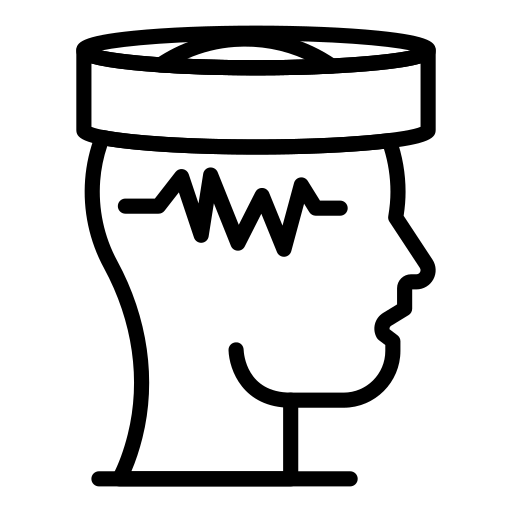
\includegraphics[width=1.5cm]{gfx/encephalography.png}};
      
            \node[below] at (A.south) (a) {\textbf{Encephalography}};

        \end{tikzpicture}
    \end{center}
\end{itemize}
\end{frame}

\begin{frame}{Norbert Wiener's Study}
    \begin{itemize}
        \item[-] First attempt with firm mathematical basis
        \item[-] Autocorrelation
    
    \end{itemize}
    \begin{block}{What is autocorrelation?}
        Mathematical tool to analyze the degree to which a signal is correlated to itself over different time shifts.\\ Formally between $f(t)$ and $f(t + \tau)$, $\tau$ = time displacement.
    \end{block}

    \begin{enumerate}
        \item Using complex functions simplifies the analysis of signals, especially wave-like signals.
        \item The time mean of the product of $f(t + \tau)$ with the complex conjugate of $f(t)$
        \item Fourier Transform of Autocorrelation: The power spectrum of $f(t)$
        
    \end{enumerate}
\end{frame}

\begin{frame}{Autocorrelation results}
 \begin{enumerate}
        \item Ink-writer vs. Magnetic tape
        \item Two playback heads
        \begin{center}
            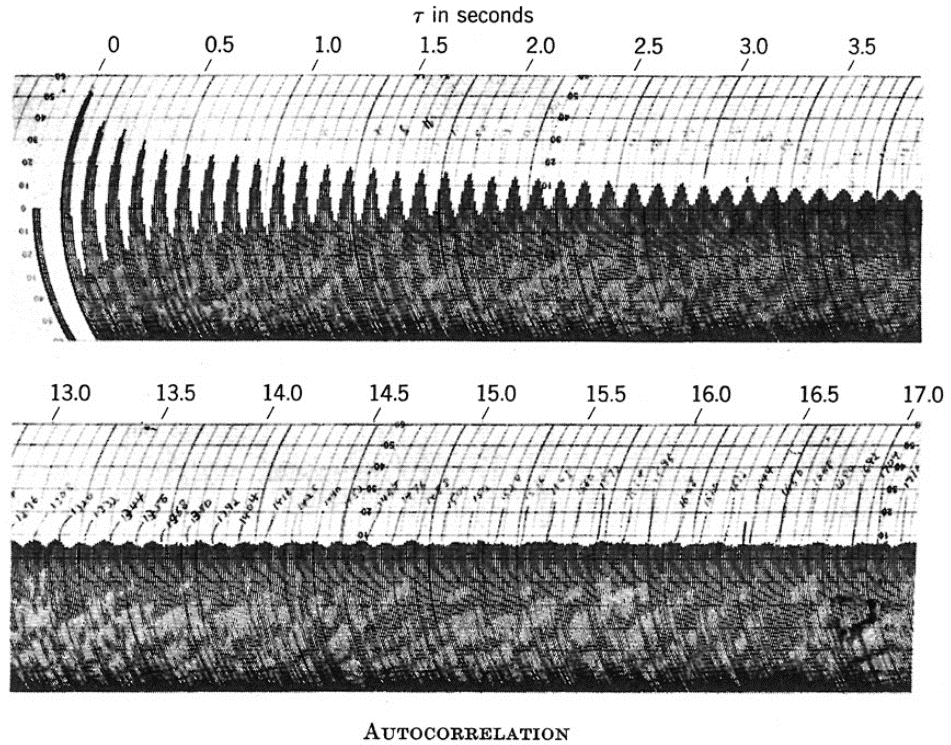
\includegraphics[width = 6cm]{png/autocorrelation.png}
        \end{center}
        
    \end{enumerate}
    
\end{frame}

\begin{frame}{Results of Harmonic Analysis}
    \begin{center}
            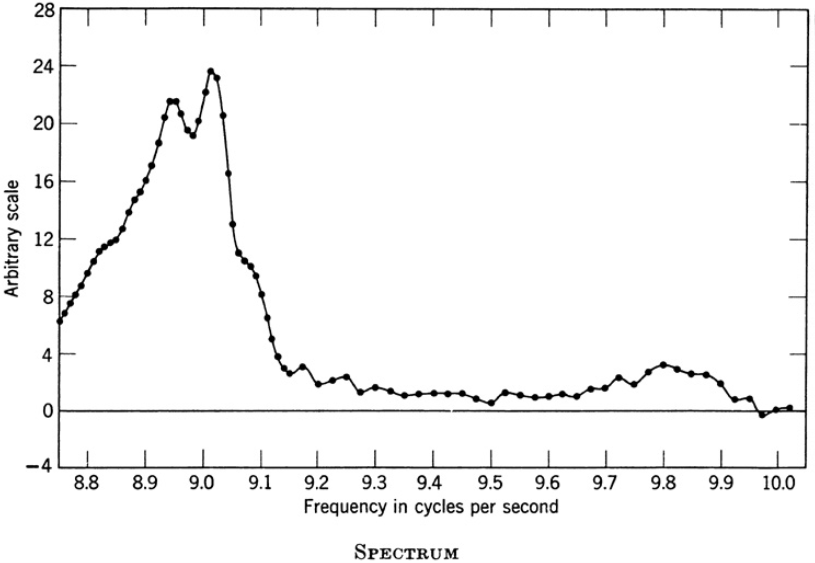
\includegraphics[width = 10cm]{png/frequencies.png}
        \end{center}
\end{frame}

\begin{frame}{Gating Mechanism in Brain Functioning}
    \begin{enumerate}
        \item Sharp Frequency Line as an Accurate Clock
        \item Clocks in Control and Computation Apparatuses
        \item Concept of Gating
        \item Combining Impulses
        \item Efficiency through Combined On-and-Off Signals
        \item Application to the Brain\\
        
    \end{enumerate}
    \begin{center}
            \begin{tikzpicture}[font=\small,scale=0.9, transform shape]
                 %\node[criminal,minimum size=1cm,monitor] (A) at (-5,0){};
                \path (-4.5,0) node(A) {
\includegraphics[width=1.5cm]{gfx/brain.png}};
                 \path (-1.5,0) node(D) {
\includegraphics[width=1.4cm]{gfx/wall-clock.png}};
                \path (4.5,0) node(B) {
\includegraphics[width=1.5cm]{gfx/cpu.png}};
                \path (1.5,0) node(C) {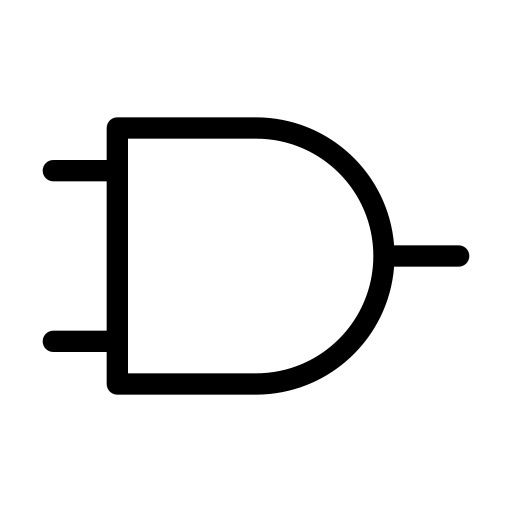
\includegraphics[width=1.5cm]{gfx/logic-gates.png}};
                \node[below] at (A.south) (a) {\textbf{Brain}};
                \node[below] at (B.south) (b) {\textbf{Computation}};
                \node[below] at (C.south) (c) {\textbf{Gating}};
                \node[below] at (D.south) (d) {\textbf{Clock}};
            \end{tikzpicture}
        \end{center}
\end{frame}

\begin{frame}{Discussion (wahrscheinlich nicht nötig)}
    \begin{enumerate}
        \item Brain Oscillators
        \item Frequency Attraction and Clumping
        \item Spectrum Gaps
        \item Supporting Evidence
        \item Biological and Non-Living Analogies
        \item Potential Research Directions
        \item Broader Implications
        
    \end{enumerate}
    
\end{frame}

\begin{frame}{Brain waves as self-organizing system}
    \begin{block}{Question: In what way is the brain/brain waves a self-organizing system?}
        \begin{enumerate}
            \item Frequency Synchronization
            \item Self-Regulation in Response to Stimuli
            \item Biological Rhythms and External Entrainment
        \end{enumerate}
    \end{block}
    
\end{frame}



\section{Project}

\begin{frame}{Pipleline}
\begin{figure}[h]
  \centering
  \begin{tikzpicture}[font=\small,scale=0.9, transform shape]
      %\node[criminal,minimum size=1cm,monitor] (A) at (-5,0){};
      \path (-4,0) node(A) {
\includegraphics[width=1.5cm]{gfx/csv-datei.png}};
      \path (0,0) node(c) {
\includegraphics[width=1.5cm]{gfx/python-datei.png}};
      \path (0,-2.5) node(b) {
\includegraphics[width=1.5cm]{gfx/python-datei.png}};
      \path (4,0) node(d) {
\includegraphics[width=1.5cm]{gfx/csv-datei.png}};	
	   \path (-4,-2.5) node(e) {
\includegraphics[width=1.5cm]{gfx/python-datei.png}};
      \path (0,-5.5) node(f) {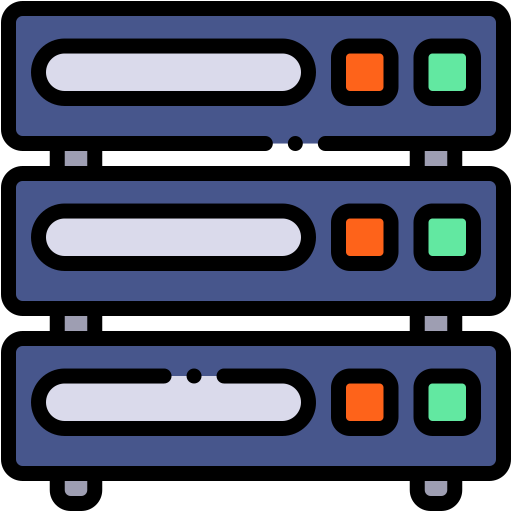
\includegraphics[width=1.5cm]{gfx/server.png}};
      \path (-4,-5.5) node(g) {
\includegraphics[width=1.5cm]{gfx/github-logo.png}};
      \path (4,-5.5) node(h) {
\includegraphics[width=1.5cm]{gfx/website.png}};

    \node[below] at (h.south) (hn) {\textbf{Website}};
    \node[below] at (g.south) (gn) {\textbf{GitHub}};
    \node[below] at (f.south) (fn) {\textbf{Cloud}};
    \node[below] at (e.south) (en) {\textbf{app.py}};
    \node[below] at (d.south) (v) {\textbf{New CSV}};
    \node[below] at (A.south) (x) {\textbf{CSV}};
	\node[below] at (c.south) (y) {\textbf{cleaner.py}};
	\node[below] at (b.south) (z) {\textbf{chatbot.py}};

	\draw[->] (A.east) --(c.west);
    \draw[<->] (f.east) --(h.west);
     \draw[->] (g.east) --(f.west);
    \draw[->] (c.east) --(d.west);
    \draw[<-] (v.south) |-(b.east);
    \draw[<->] (e.east) -- (b.west);
	%\draw[<->] (y.south) |- (b.east);
	%\draw[->] (x.south) -- (b.west);
  \end{tikzpicture}
  \caption{Schema of Express}
\end{figure}
\end{frame}

\begin{frame}{Machine Learning - Work Flow}
    \begin{enumerate}[1)]
      \item \textbf{Feature Selection:} stars, director, genre, year, runtime.
\item \textbf{Data Preprocessing:} Convert categorical data to numeric with LabelEncoder.
\item \textbf{Target Categorization:} Metascore $\mapsto$ 'Low,' 'Medium,' 'High,' and 'Very High.'
\item \textbf{Model Training:} Train DecisionTreeClassifier with preprocessed data.
\item \textbf{Model Evaluation:} Test and evaluate the model's accuracy with metrics.
\item \textbf{Prediction:} Input movie features to predict the Metascore category.
\item \textbf{Recommendation:} Filter \& recommend movies based on the predicted category.
    \end{enumerate}
\begin{block}{Input - Predict - Output}
    %Decision trees make decisions by asking a series of yes/no questions about the features of a dataset. This process is inherently categorical, as each question splits the data based on category-like criteria.
Based on the users' input, the trained model predicts a new Raiting and then gives the movie title of the predicted Raiting. 
\end{block}
\end{frame}

\begin{frame}{Decision Tree}
\begin{figure}
\centering
\begin{tikzpicture}[auto,
                    box/.style={draw, rectangle, minimum size=3em, text centered},
                    line/.style={draw, -Latex}]
    % Nodes
    \node [box]                                     (root)     {Root};
    \node [box, below=0.5cm of root, xshift=-3cm]   (genreA)   {Drama};
    \node [box, below=0.5cm of root, xshift=3cm]    (genreO)   {Action};
    \node [box, below=0.5cm of genreA, xshift=-1cm] (actorA)   {Actor: A};
    \node [box, below=0.5cm of genreA, xshift=1cm]  (actorB)   {Actor: B};
    \node [box, below=0.5cm of genreO, xshift=-1cm] (runtime1) {95};
    \node [box, below=0.5cm of genreO, xshift=1cm]  (runtime2) {95};
    \node [box, below=0.5cm of actorA]              (high)     {High};
    \node [box, below=0.5cm of actorB]              (medium)   {Medium};
    \node [box, below=0.5cm of runtime1]            (low)      {Low};
    \node [box, below=0.5cm of runtime2]            (medhigh)  {High};
    
    % Paths
    \path [line] (root) -| (genreA);
    \path [line] (root) -| (genreO);
    \path [line] (genreA) -- (actorA);
    \path [line] (genreA) -- (actorB);
    \path [line] (genreO) -- (runtime1);
    \path [line] (genreO) -- (runtime2);
    \path [line] (actorA) -- (high);
    \path [line] (actorB) -- (medium);
    \path [line] (runtime1) -- (low);
    \path [line] (runtime2) -- (medhigh);
\end{tikzpicture}

\end{figure}
\end{frame}
\section{Performance}
\begin{frame}{Confusion Matrix}
    \begin{figure}
        \centering
        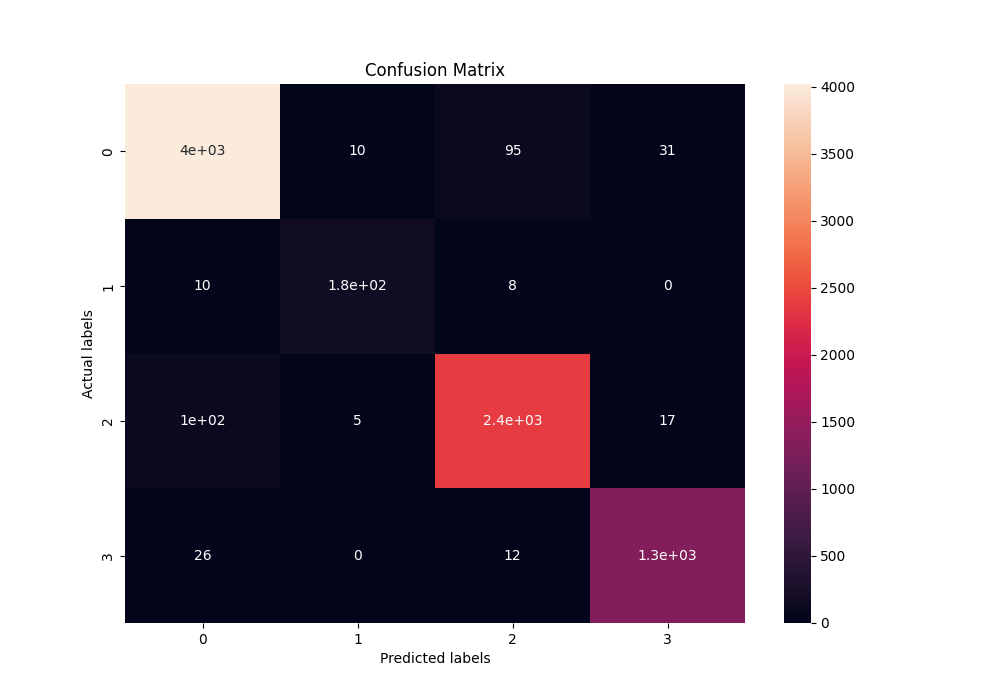
\includegraphics[width=.7\textwidth]{png/confusion_matrix.png}
        \caption{Caption}
        \label{fig:enter-label}
    \end{figure}
Shows the classification TP, FP, FN, TN\newline
TP: 1300 \hfill FP: 48 \hfill FN: 38 \hfill TN: 6808 
\end{frame}

\begin{frame}{Classification Report}

    \begin{block}{What is what?}
        \begin{enumerate}[\indent$\square$]
            \item \textbf{Precision:} Ability of a classifier not to label an instance positive that is actually negative.
            \item \textbf{Recall:} Ability of a classifier to find all positive instances.
            \item \textbf{F1 Score:} A weighted average of precision and recall. An F1 score reaches its best value at 1 (perfect precision and recall) and worst at 0
            \item \textbf{Macro average} computes the average metric (precision, recall, F1-score) for each class equally, regardless of class size 
            \item \textbf{Weighted average} takes the class size into account, giving more weight to larger classes
        \end{enumerate}
    \end{block}
Mapping 0: $\mapsto$ Low,\hfill 1: $\mapsto$ Medium,\hfill 2: $\mapsto$ High,\hfill 3: $\mapsto$ Very High   
\end{frame}
\begin{frame}{Pre-Re-F1 (Not Formula one) - What?}
\begin{table}
\caption{Classification Report}
\begin{tabular}{p{2cm} p{1.5cm} p{1.5cm} p{1.5cm} p{1.5cm}}
\hline 
\textbf{class} & \textbf{precision} & \textbf{recall} & \textbf{f1\_score} & \textbf{support} \\
0 & 0.97 & 0.97	& 0.97 & 4155 \\
1 & 0.92 & 0.91	& 0.91 & 195 \\
2 & 0.95 & 0.95	& 0.95 & 2498 \\
3 & 0.97 & 0.97	& 0.97 & 1376 \\
\\
macro avg & 0.95 & 0.95 & 0.95\\
weighted avg & 0.96 & 0.96 & 0.96 \\
\hline 
\end{tabular}
\end{table}
    $\Rightarrow$ With high macro (0.95) and weighted (0.96) averages in precision, recall, and F1-score, the model shows excellent overall performance, indicating that \underline{both} \textbf{the model} and \textbf{dataset} are well-suited for the task.
    \end{frame}
\begin{frame}{Project}
\begin{figure}
    \centering
    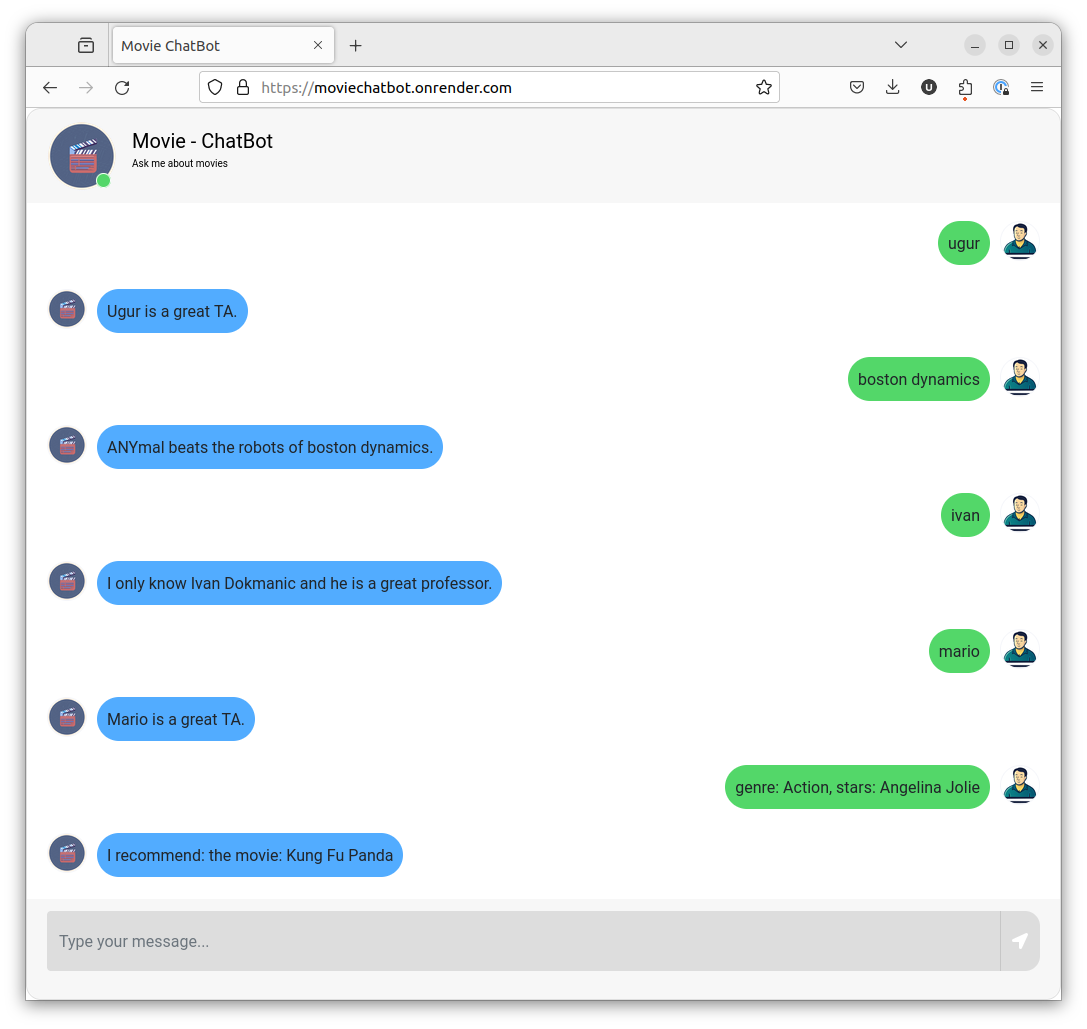
\includegraphics[width=0.65\textwidth]{png/result-correct.png}
    \caption{Our Project result}
    \label{fig:enter-label}
\end{figure}
\end{frame}
\end{document}
